\section{Quadtree-based methods}\label{sec:quadtree}

Today, the dissemination of gridded data is becoming widespread, as it allows for adjusting the scale at which information is made available. Additionally, a grid is a purely geometric and regular partitioning independent of administrative boundaries. Gridded data generally allows for better consideration of scale and zoning effects underlying the Modifiable Areal Unit Problem (MAUP) theorized by \cite{openshaw1979million}.

However, gridding also provides an opportunity to disseminate information about increasingly smaller geographical areas. For example, Insee (French National Institute of Statistics and Economic Studies) disseminates certain tax information on grids of 200m square\footnote{\url{https://www.insee.fr/fr/statistiques/7655475?sommaire=7655515} (in French)}, and all European statistical institutes are preparing to disseminate population data from the 2021 Census on 1km $\times$ 1km grids. This increases the risks of reidentification or disclosure of sensitive attributes. Without adequate protection methods, the dissemination of such data would not be possible.

To mitigate the risks of disclosure, a population threshold is generally set so that below it, information is considered sensitive or confidential and must be treated.

Among the non-perturbative methods available to the producer, \citet{Strobl_2005}, for the dissemination of Austrian Census data, and \citet{Behnisch_Meinel_Tramsen_Diesselmann_2013}, for the Leibniz Institute, have proposed using the so-called \emph{quadtree method} to protect gridded data from the risk of disclosing confidential information. This technique has also been implemented by \citet{Lagonigro_Oller_Martori_2017} and \citet{Suñé_Ibáñez_2017} for the Statistical Institute of Catalonia, and a variant is used by Insee \citep{Branchu_Costemalle_Fontaine_2018} for the dissemination of tax data and Census 2021 results.


\subsection{The aggregation process}

The Quadtree is primarily a space subdivision technique proposed by \cite{hunter1978efficient} and further developed by \cite{Samet_1984}, which relies on a hierarchical structure of space in the form of nested grids of increasingly larger resolutions.

\begin{tcolorbox}[breakable]
Taking an example from \cite{Lagonigro_Oller_Martori_2017}, shown here as Fig.~\ref{fig:subdivision_quadtree}, $A$ represents the maximum extent of the map as a single grid. The size of this grid defines the lowest possible resolution. This grid is subdivided into $4$ grids of medium resolution ($B$, $C$, $D$, and $E$), and $C$ is further subdivided into 4 grids of maximum resolution ($F$, $G$, $H$, and $I$). This decomposition can also be represented as a hierarchical tree, hence the name of the method.

%\begin{figure}
    %\centering
    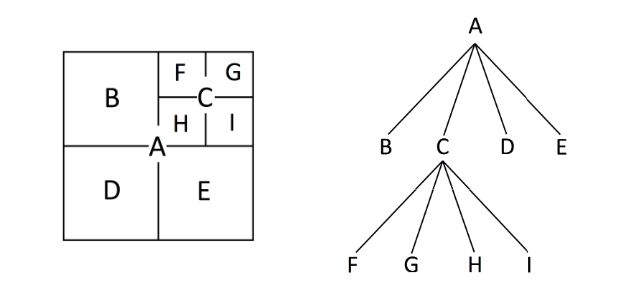
\includegraphics[width=0.8\linewidth]{figures/Quadtree/space_subdivision_lagonigro_fig1.png}
    \captionof{figure}{Subdivision of space and its equivalent quadtree representation (Source: \cite{Lagonigro_Oller_Martori_2017}, p. 144).}
    \label{fig:subdivision_quadtree}
%\end{figure}
\end{tcolorbox}

As a data protection technique, the quadtree involves disseminating each non-confidential information at the highest desired resolution level. The hierarchical tree can be built using two types of approaches:
\begin{itemize}
\item A \emph{bottom-up} approach, by far the most common, starting from the maximum resolution level (the leaves of the tree) and aggregating grids in the presence of confidential information;
\item A \emph{top-down} approach would start from the minimum resolution level (root of the tree) and decompose each grid until a confidential information is disclosed.
\end{itemize}

\cite{Behnisch_Meinel_Tramsen_Diesselmann_2013} and \cite{Lagonigro_Oller_Martori_2017} both use a fairly similar bottom-up approach.

We will use the example presented in Figure~\ref{fig:quadtree_aggregation} to detail the steps of the aggregation algorithm. We assume that the territory is divided into four levels of resolution: 250~m $\times$ 250~m (resolution 1, thin gray lines), 500~m $\times$ 500~m (resolution 2, thin black lines), 1~km $\times$ 1~km (resolution 3, thick black lines), and 2~km $\times$ 2~km (resolution 4, thick blue lines). This example is adapted from Figure 14.2 in \citet[p.358]{BuronFontaine2018}. In this example, the confidentiality threshold is set to $3$: each cell must contain at least three individuals to be disseminated.

\begin{figure}
    \centering
    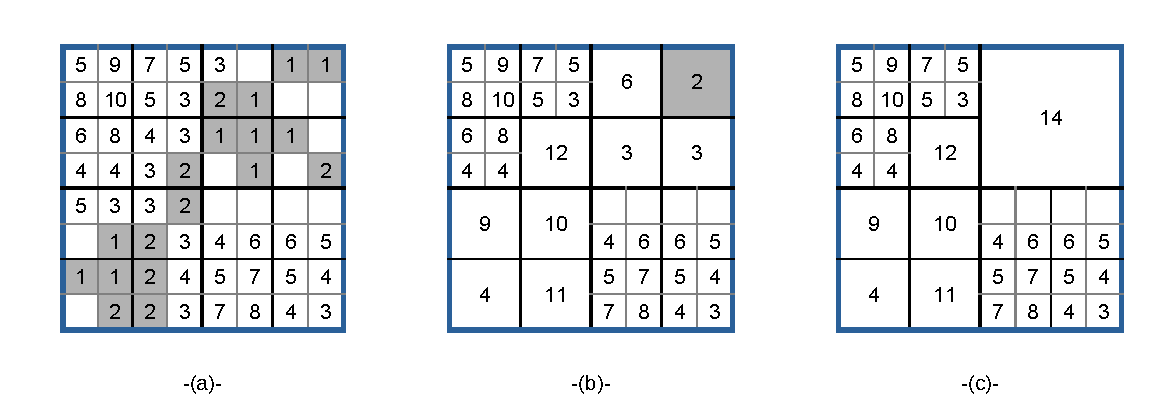
\includegraphics[width=1\linewidth]{figures/Quadtree/adaptation_example_handbook_spat_ana.pdf}
    \caption{Quadtree aggregation with a bottom-up approach (confidentiality threshold $=3$) - adapted from \citet[p.358]{BuronFontaine2018}}
    \label{fig:quadtree_aggregation}
\end{figure}

\begin{itemize}
    \item First, the information is distributed in the grid with the finest possible resolution (resolution 1, Figure~\ref{fig:quadtree_aggregation} (a)). All cells containing confidential information are identified (gray cells).
    \item Each confidential cell is aggregated with the other three cells belonging to the same resolution 2 cell. Thus, at the bottom left, the information is no longer disseminated at resolution 1 but will be at best at resolution 2 (Figure~\ref{fig:quadtree_aggregation}, (b)).
    \item Since there is still a resolution 2 cell below the confidentiality threshold (top right), it is necessary to aggregate this cell with the other three cells belonging to the same resolution 3 cell (Figure~\ref{fig:quadtree_aggregation}, (c)).
    \item The grid (c) no longer contains confidential information and can be disseminated.
\end{itemize}

\subsubsection{Choice of the grid and anchoring of the hierarchical structure}

The quadtree approach relies on a hierarchical structure of grid cells. This means that this method can only be applied if the areas of a specific resolution are perfectly nested within each of the areas of higher resolutions. For example, a quadtree can't be achieved with a $200$~m and a $500$~m grid at the same time, because not all the $200$~m squares are entirely contained in a $500$~m square.\bigskip

Although a strict quadtree approach consists of splitting each square into four smaller squares, it is possible to design a variant that first chooses the size of the different resolution levels and then applies a quadtree to all the chosen resolutions. For example, it is possible to adapt the methodology so as to release $100$~m squares as the lowest resolution, and $500$~m and $1$~km squares as intermediate resolutions if necessary. In this case, with a bottom-up approach, within a given $500$~m square, the information is released at the $100$~m resolution if and only if all of the twenty-five $100$~m squares are above the threshold.\bigskip

In addition, the result of the aggregation process is highly dependent on the anchoring of this hierarchical structure. A slight shift in one or more directions can have significant consequences for the method's output. Based on the example presented earlier (Fig.~\ref{fig:quadtree_aggregation}), suppose we keep exactly the same population per cell (finest grid in gray) but shift the anchoring of the hierarchical structure (black lines, dark black, and thick blue) by one cell downwards and one cell to the right. The new aggregation process is shown in Figure~\ref{fig:quadtree_pos_grid}. It can be observed that this leads to very different results, requiring, in particular, the aggregation of two very large cells (bottom left and top right), resulting in significant information loss.

\begin{figure}[ht]
    \centering
    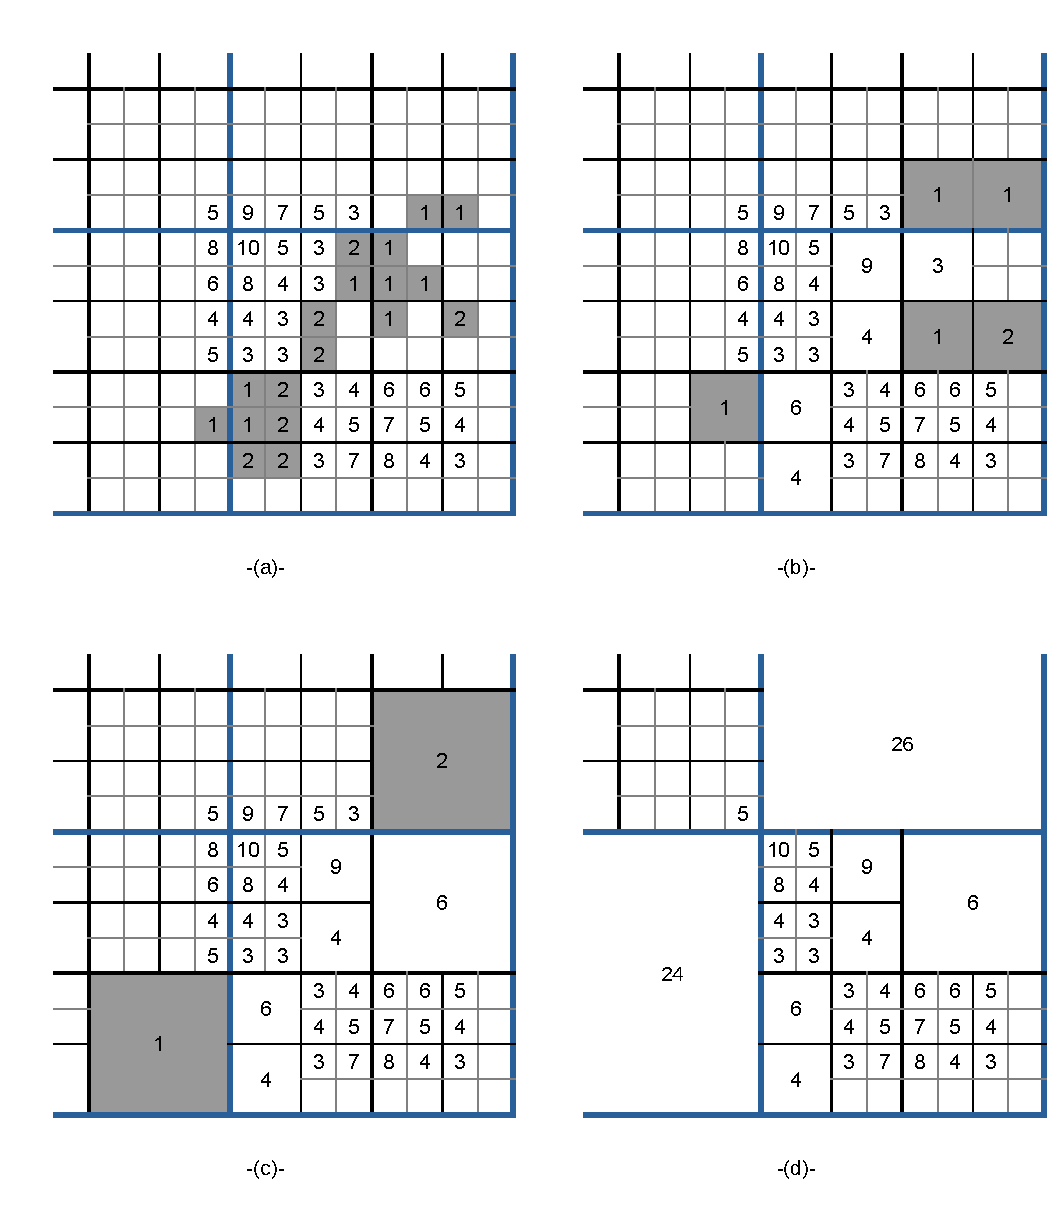
\includegraphics[width=0.89\textwidth]{figures/Quadtree/adaptation_example_variante_pos_grid.pdf}
    \caption{Quadtree applied on the same population as in Fig.~\ref{fig:quadtree_aggregation}, but with a different anchoring of the hierarchical structure}
    \label{fig:quadtree_pos_grid}
\end{figure}

One could consider testing several positions of the hierarchy (but taking also the  spatial hierarchy formally assumed for publication purposes into account) and choosing the one that leads to the minimal information loss. However, such a solution would have the major drawback of making maps (for example, from one year to another) impossible to compare. In the context of a single study, this option could be considered, but it does not seem realistic for the work of a statistical institute.

Instead, it is more beneficial, following the examples of \cite{Behnisch_Meinel_Tramsen_Diesselmann_2013} and \cite{Lagonigro_Oller_Martori_2017}, to use the INSPIRE grid coding standard. This standard ensures perfect stability of the grid cells and their hierarchical structure. This allows tools such as the R packages \texttt{sdcSpatial} \citep{sdcSpatial_2022} and \texttt{AQuadtree} \citep{AQuadtree_2023} to provide stable results. However, this choice does not guarantee the minimization of information loss during the quadtree process.


\subsubsection{Resolution Levels}

The bottom-up approach begins with a maximum resolution level, i.e., with the smallest tiles desired by the producer. The method iteratively changes the resolution level of the information to be disseminated as long as there is confidential information remaining. The classic choice is to select a resolution twice as low at each iteration: starting with tiles of $250$~m, the next level would consist of tiles of $500$~m, then $1$~km, and so on. This is the choice made by \citet{Behnisch_Meinel_Tramsen_Diesselmann_2013} and \citet{Lagonigro_Oller_Martori_2017}, and it is the one implemented in \citet{sdcSpatial_2022} as well as \citet{AQuadtree_2023}. In this case, each tile at a higher level consists of exactly 4 tiles at the lower level. However, in theory, there is no restriction on pre-selecting resolution levels. For example, Insee has chosen a maximum resolution of $200$~m $\times$ $200$~m, with the higher level being $1$~km $\times$ $1$~km. This higher level thus contains $25$~tiles of $200$~m, which may lead to a more significant local information loss than with a classic hierarchy.

In the absence of pre-defined stopping criteria, the aggregation process will continue as long as a tile contains confidential information. The R package \texttt{sdcSpatial} \citep{sdcSpatial_2022} suggests setting the minimum acceptable resolution level. It is therefore possible to choose to stop the aggregation process before all confidential cells are processed, with a complementary (suppressive or perturbative) method being considered additionally.

\subsubsection{Extreme Cases of Aggregation}

Setting a minimal acceptable resolution level turns out to be a good idea to prevent some rare but extreme situations from excessively altering the data's utility. Figure~\ref{fig:quadtree_reunion} shows a quadtree applied to household numbers on the French island of La Réunion. This volcanic island has its population mainly located on the coast. 

The quadtree is applied starting from a $200$~m grid, then a $1$~km, $2$~km grid, and so on. However, applied without a stopping criterion, we observe that the aggregation process leads to the formation of $3$ tiles of $16$~km each, with an average of over $17,000$ households. The information loss is significant and is actually due to very specific configurations. The case of the tile surrounded in red is presented in Figure~\ref{fig:quadtree_reunion_issue}, where the $1$~km tiles have been represented, along with the $4$~tiles of $8$~km composing the red tile in Figure~\ref{fig:quadtree_reunion}. It can be observed that the southeast quarter consists of only two $1$~km tiles, each containing at most $4$~households. In total, these two tiles count at most $8$~households, which is below the authorized dissemination threshold of $11$~households.\footnote{
    We reassure the reader that in reality this information is not confidential and can be used here for demonstration purposes.}

Thus, aggregating these two tiles at the $8$~km resolution level is not sufficient and requires aggregation at a lower resolution level ($16$~km). However, it turns out that this tile is adjacent to a densely populated area, resulting in the complete loss of detail of the dense part of this area.

\begin{figure}[H]
\begin{minipage}{0.48\linewidth}
    \centering
    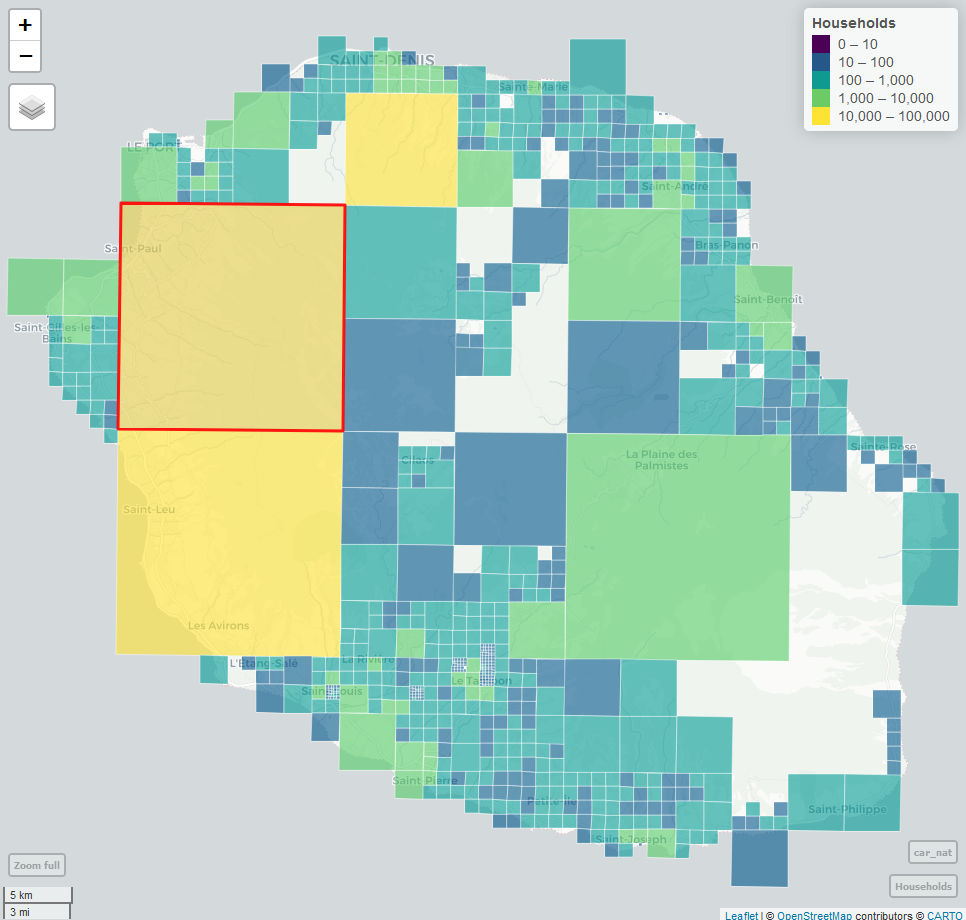
\includegraphics[width=\linewidth]{figures/Quadtree/reunion_quadtree_filo2019.png}
    \caption{Quadtree approach applied on household numbers in La Réunion (France)}
    \label{fig:quadtree_reunion}
\end{minipage}
\hfill
\begin{minipage}{0.48\linewidth}
    \centering
    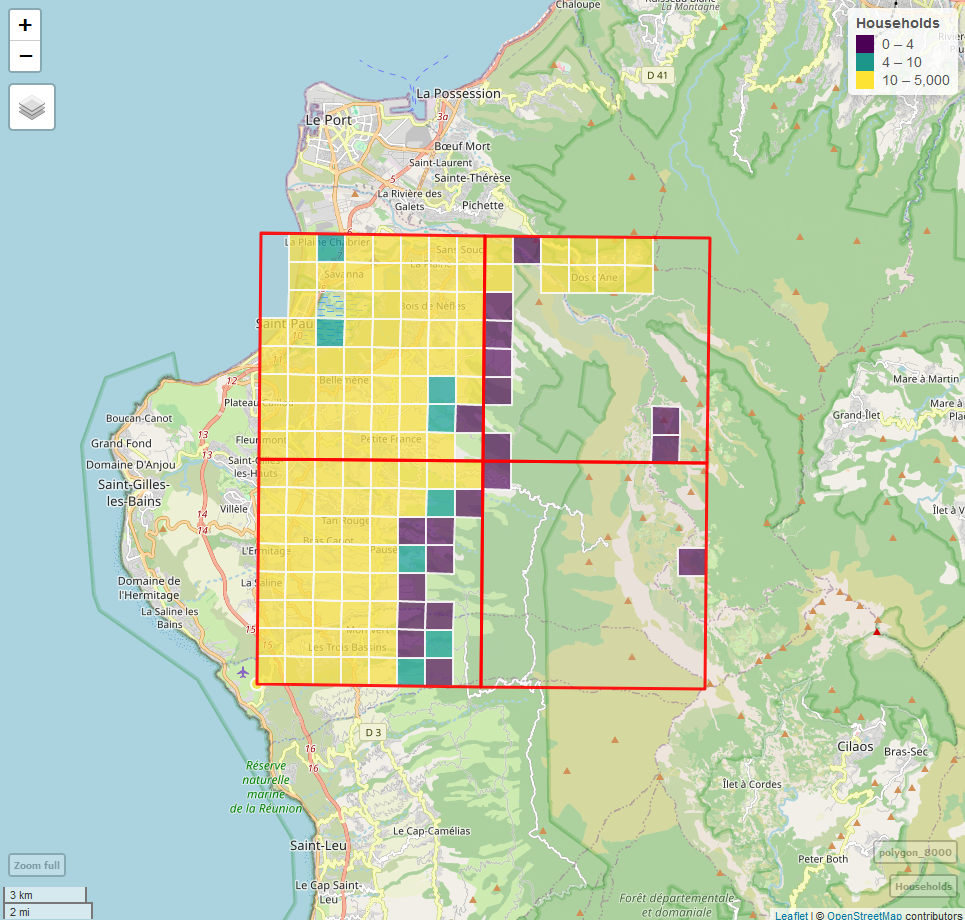
\includegraphics[width=\linewidth]{figures/Quadtree/reunion_quadtree_filo2019_issue.png}
    \caption{Quadtree issue in extreme case\\ \ }
    \label{fig:quadtree_reunion_issue}
\end{minipage}
\end{figure}

\begin{table}[H]
\footnotesize
\centering
\begin{tabular}[t]{rrrrrr}
\toprule
\multirow{2}{*}{Size of squares (meters)} & \multicolumn{2}{c}{Squares} & \multicolumn{3}{c}{Households} \\
\cmidrule{2-3} \cmidrule{4-6}
 & NB & \% & Total & \% & Mean \\
\midrule
200 & 157 & 22 & 9~662  &  3 & 62\\
1~000 & 447 & 64 & 17~8400 & 55 & 399 \\
2~000 & 64 & 9 & 32~074 & 10 & 501 \\
4~000 & 29 & 4 & 30~747 & 10 & 1~060\\
8~000 & 6 & 1 & 19~373 & 6 & 3~229\\
\addlinespace
16~000 & 3 & 0 & 52~408 & 16 & 17~469\\
ALL & 706 & 100 & 322~664 & 100 & 457\\
\bottomrule
\end{tabular}
\caption{Results of the quadtree process on households frequencies in La Réunion}
\label{tab:quadtree_reunion_summary}
\end{table}


Such cases justify an approach consisting of setting a minimal resolution level, even if it means having to deal separately with the untreated confidential tiles. A suppressive method, consisting of removing the information from the remaining confidential tiles ,is a feasible option (see section \ref{sec:aux_suppr}). The information loss is generally not significant, since it concerns only tiles below the confidentiality threshold. \citet{Lagonigro_Oller_Martori_2017} and \citet{Suñé_Ibáñez_2017} choose to randomly relocate the population of these tiles. \citet{Suñé_Ibáñez_2017}, in particular, demonstrates the usefulness of this approach in terms of utility through simulation studies.


\subsection{Utility Aspects}

% Show that utility decreases with the aggregation level
Using the Hellinger distance (see \ref{sec:util_DD_hd}) or the Kantorovich-Wasserstein distance (see \ref{sec:util_DD_kwd}), \cite{GussenbauerEtAl2023} demonstrated on several examples that at the same protection level, the quadtree method resulted in a stronger loss of information compared to a method of removing cells containing confidential information, but less significant than smoothing.

By choosing a minimal resolution level in advance, the same article shows the expected effect on utility: by allowing the aggregation of confidential cells at an additional level, the Hellinger distance increases significantly in most cases. This experimentation illustrates the importance of setting a minimal resolution level as a stopping criterion for the aggregation process to maintain good utility. However, such a choice requires additional measures to protect any remaining confidential cells.

\subsubsection{Quadtree and Spatial Analysis}

Spatial autocorrelation is an essential element of spatial analysis. To provide useful spatial data, care must be taken to ensure that the protection mechanism does not overly alter the intensity of the initial autocorrelation. However, the quadtree, by aggregating certain cells, will distort the intrinsic neighborhood relationships. Let's take the example of households residing on the island of La Réunion (Fig.~\ref{fig:quadtree_reunion}). After aggregation, Moran's $\mathcal{I}$ (see section \ref{sec:util_moran}) is $0.228$, whereas it was $0.555$ on the original data for a $1$~km grid (Tab.~\ref{tab:MoranI_reunion}). Worse, using Euclidean distance to define neighbor weights, Moran's $\mathcal{I}$ becomes very close to $0$ ($0.050$). Although the statistic remains significantly different from zero, the data disseminated with the quadtree method reduces the importance of the observed spatial autocorrelation.

Such distortion can be controlled by avoiding extreme cases of aggregation, especially by limiting the acceptable minimal resolution level and separately processing the remaining extreme cases (see above). Limiting the minimal resolution level will also prevent the reappearance of scale issues (MAUP) in data analysis.

\begin{table}
    \centering
    \begin{tabular}{ccc}
        \toprule
        \multirow{2}{*}{Release} & \multicolumn{2}{c}{Moran's $\mathcal{I}$} \\
        \cmidrule{2-3}
                                 & Queen Neighbor & Euclidian distance\\
        \midrule
        original 1km grid        & 0.555          & 0.331 \\
        maximal quadtree         & 0.228          & 0.050 \\
        \bottomrule
    \end{tabular}
    \caption{Moran's $\mathcal{I}$ applied on household frequencies in La Réunion, depending on the release and the way to define the neighborhood.}
    \label{tab:MoranI_reunion}
\end{table}
% All test statistics are significant at the 5% level.

\subsubsection{How to Disseminate Multiple Variables on Comparable Maps?}

The quadtree is theoretically a method to be applied separately for each variable we want to disseminate. However, there is no guarantee that the process will lead to the same result in terms of aggregation. Worse, it is even expected that the results will be different. Thus, maps become hardly comparable and lose their utility. What should we do, if we want to disseminate maps of total population, female population, and male population in a given territory and allow comparability of published maps?

\cite{Lagonigro_Oller_Martori_2017} propose setting a second threshold they call the \emph{anonymity threshold}, in addition to the \emph{aggregation threshold}. The latter determines whether the tiles should be aggregated or not, while the former specifies whether attribute information can be disseminated or not. If a tile meets the aggregation threshold but not the anonymity threshold for one of its attributes, the overall information (total population) is then disseminated but the information on the attribute in question is to be suppressed. A secondary suppression is also necessary to avoid differencing with margins. Thus, a suppression step is applied to the attributes.

For example, let's suppose that in a given tile there are $10$~inhabitants, of which $2$ are men. Suppose further that the aggregation level is set to $9$ and the anonymity threshold to $3$. In this case, the aggregation process won't aggregate the tile to a lower resolution level and the total population of the tile will be disseminated. But the number of men won't be released, because it is below the anonymity level. In order to avoid any margin differencing, one has to suppress the counts of females too.

 For the authors, this anonymity threshold applied to attributes ensures a protection level compliant with $k$-anonymity. It is actually an extensive version of $k$-anonymity, where all disseminated attributes would be considered quasi-identifiers.

The disadvantage of this method is that it requires choosing two thresholds, the aggregation threshold having to be higher than the anonymity threshold of the attributes. For example, it is possible to choose an aggregation threshold based on the anonymity threshold chosen beforehand. \cite{Lagonigro_Oller_Martori_2017} show that by increasing the aggregation threshold, the loss of precision, measured by the proportion of maximum resolution tiles retained, is compensated by the decrease in information loss caused by the suppression of attributes below the anonymity threshold.

A method based on the quadtree, but injecting a dose of perturbation, is presented below (section~\ref{sec:variante_insee}).

\subsection{Risk Aspects}

\subsubsection{Quadtree and geographic differencing}

As a non-perturbative method, the quadtree does not protect against the risk of geographical differencing (described in section \ref{sec:risk_diff}). It is therefore necessary to manage this differencing risk in a second step, if the information is also disseminated on other zoning systems, such as administrative zonings, for example.

To manage this differencing risk, Insee adopted two different strategies:

\begin{itemize}
    \item For the dissemination of tax data, the institute ensured that the same information was not disseminated in grids as in other zoning systems. Geographic differencing is therefore rendered ineffective.
    \item For the dissemination of Census 2021 gridded data, this strategy could not work, as much of the information was already disseminated at the municipal level in particular. Therefore, after the quadtree method, detection and treatment of cases of geographic differencing were carried out using the R package \texttt{diffman} \citep{diffman} (see also section \ref{sec:risk_diff_diffman}).
\end{itemize}


\subsection{Tools}

\begin{figure}[H]
\begin{minipage}{0.48\linewidth}
Two R packages, \texttt{sdcSpatial} \citep{sdcSpatial_2022} and \texttt{AQuadtree} \citep{AQuadtree_2023}, implement a protection process based on the quadtree approach. Both packages take point-based geographical data as input, create grid cells, and build the quadtree based on the desired minimum and maximum resolution levels. Both packages are also consistent with the INSPIRE geocoding norm. \bigskip

However, they differ in how they present the final information: \texttt{sdcSpatial} represents a grid of cells at the finest desired (maximal) resolution level: at the end of the quadtree, the aggregated information is equally redistributed across all cells of the maximal resolution (Fig.\ref{fig:quadtree_sdcspatial_result}). In contrast, \texttt{AQuadtree} represents a grid with cells of different sizes, depending on the resolution level achieved by the aggregation process.
\end{minipage}
\hfill
\begin{minipage}{0.48\linewidth}
    % \begin{figure}
    % \centering
    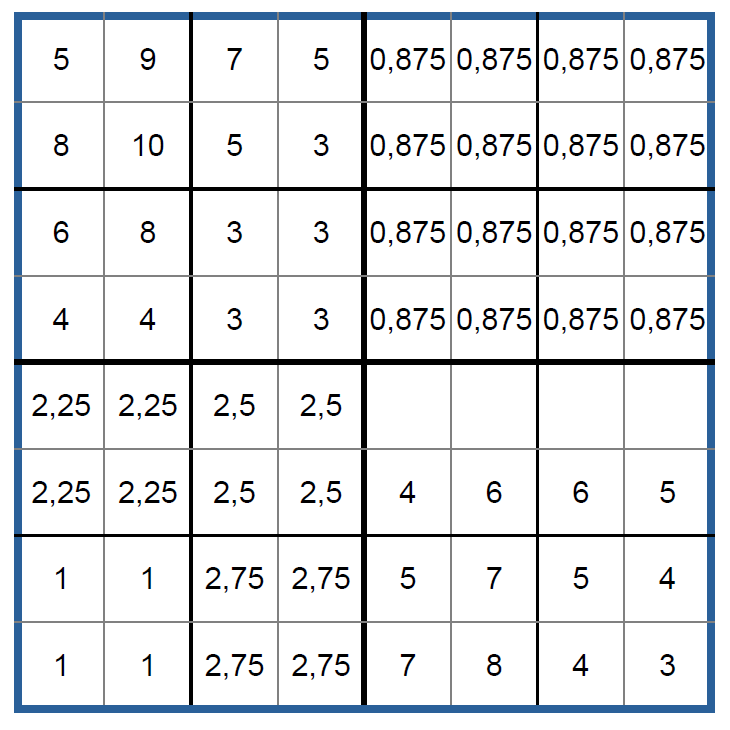
\includegraphics[width=\linewidth]{figures/Quadtree/adaptation_example_variante_sdcspatial_fix.png}
    %\vspace{-0.5cm}
    \caption{Result of \texttt{sdcSpatial} if applied on the grid of the example displayed in Fig.\ref{fig:quadtree_aggregation}.}
    \label{fig:quadtree_sdcspatial_result}
    % \end{figure}
\end{minipage}
\end{figure}




\subsection{A variant of the quadtree approach developped at Insee}\label{sec:variante_insee}


Insee has developed a method based on the quadtree to disseminate data from tax sources on a grid of $1$~km cells and another grid of $200$~m cells \citep{Branchu_Costemalle_Fontaine_2018}. This method has been implemented in the R package called \texttt{gridy} \citep{gridy}. 

The peculiarity of this dissemination is that the counts (population and number of households) are not confidential, but their breakdowns (by sex, by age, etc.) or the sum of individual incomes, the number of households living below the poverty line, etc. are subject to confidentiality rules. The method is also used by Insee for disseminating Census 2021 data on $1$~km cells. The confidentiality rule applied here is to not disseminate original information (other than the count) on cells containing fewer than $11$ households.

\subsubsection{How does it work?}

The quadtree is used in a top-down approach: the aggregation process starts from the minimal resolution level, i.e., the one at which no cell is below the threshold.

The idea is to gather risky tiles with other ones (and also with some non-risky tiles) so as to ensure that each group contains more households than the required threshold. The process begins from the coarsest level ($64$~km) and continues to the finest one ($200$~m). The groups are inherited from one level to the next, as shown in Figure~\ref{fig:multilayer_grid}. The top-down approach lets one refine the composition of the groups to avoid the aggregation of more cells than needed for the protection. At the end of the quadtree process, we get either original cells at the desired resolution ($1$~km for example) or groups of suppressed cells.

In fact, the suppression process is just temporary. Attribute counts at the group level are distributed among the cells on a \textit{pro rata} basis of the cell's population share in the group's population. The population of the cell, which is non-confidential information, thus serves as the key for distributing other attributes.

Consider a group of cells in which we wish to proceed with the imputation of the number of males and females in each of its cells.

Let the notations be:
   \begin{itemize}
    \item $P^c$, $P^c_f$, $P^c_m$, respectively, the total population, the number of women, and men actually living in the cell $c$;
    \item $\hat{p}^c$, $\hat{p}^c_f$, $\hat{p}^c_m$, their disseminated equivalents (after allocating);
    \item $P^g$, $P^g_f$, $P^g_m$, their equivalents at the level of group $g$.
\end{itemize}

The allocation principle consists of disseminating the following values:

\begin{equation}
\begin{split}
    \hat{p}^c_m &= P^g_m \cdot \frac{P^c}{P^g} \\
    \hat{p}^c_f &= P^g_f \cdot \frac{P^c}{P^g}    
\end{split}    
\end{equation}

Thus, the total population of cell $c$ after proportional allocation is indeed equal to the original population:

\begin{equation}
    \hat{p}^c = \hat{p}^c_f + \hat{p}^c_m = \frac{P^c}{P^g} \cdot (P^g_f + P^g_m) 
    = \frac{P^c}{P^g} \cdot P^g 
    = P^c
\end{equation}

\begin{figure}[H]
    \centering
    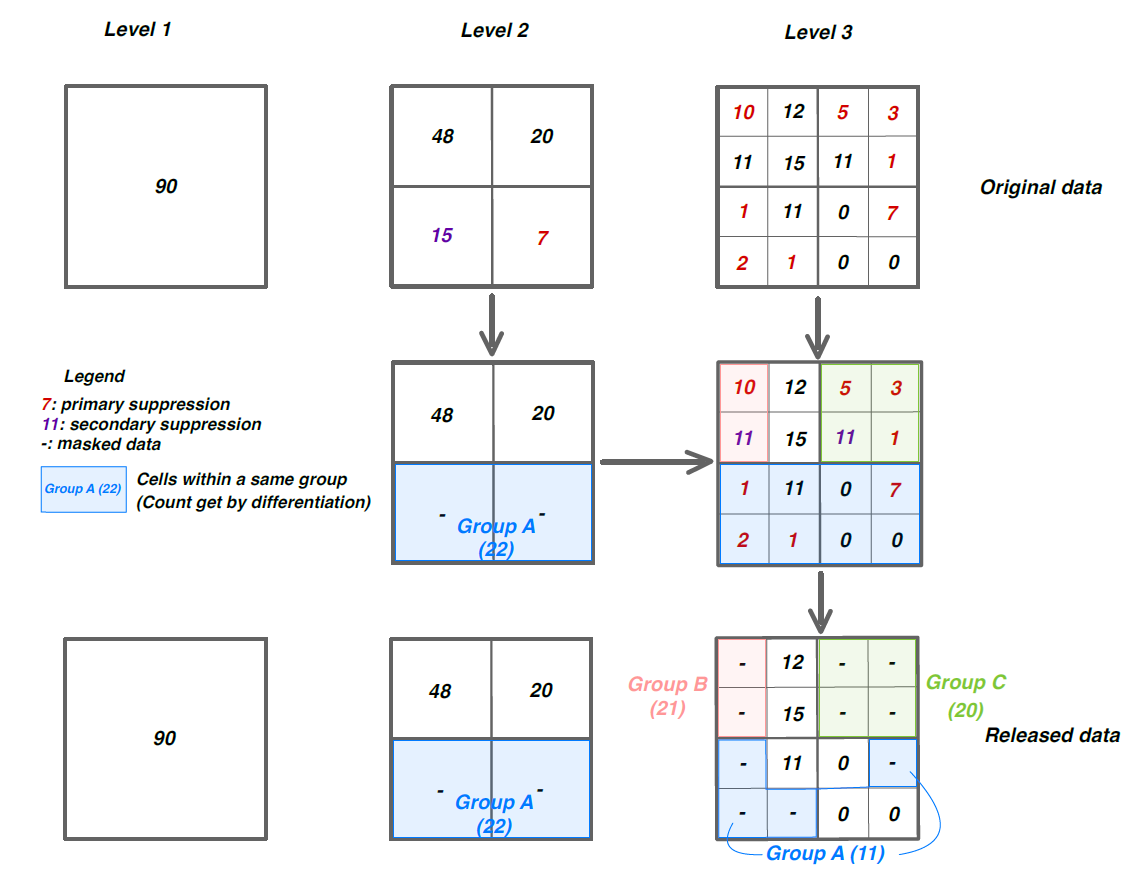
\includegraphics[width=\textwidth]{figures/Quadtree/grille_creu_proc_all.png}
    \caption{Building groups of risky tiles along a quadtree decomposition}
    \label{fig:multilayer_grid}
\end{figure}

\subsubsection{Risk and Utility aspects}

The method allows for handling the risk of attribute disclosure, and it is entirely conceivable to also address the risk of disclosure by inference by assigning one of the groups formed during the quadtree process to cells that would be too homogeneous on a (sensitive) attribute.

Nevertheless, this method  requires a variable used as a distribution key. It could then be useful when counts (population or households, for example) are not considered confidential, as is the case for population enumeration in France.

As this method is not a full perturbative one, it doesn't ensure a full protection against geographic differencing. Hence, some techniques presented in the section~\ref{sec:risk_diff} have to be applied.
In France, $78$\% of the $200$~m cells and $52$\% of the $1$~km cells are below the confidentiality threshold. 

In terms of utility, the method is quite interesting compared to a standard quadtree (Tab.~\ref{tab:insee_hell_kwd}; for the measures used see section \ref{sec:util_DD}). Indeed, it avoids aggregations over large cells or the suppression of a large amount of information.

It also preserves spatial structures in the case of the French release of Census 2021 data on a $1$~km grid, as seen in Fig.\ref{fig:moran-depts}: the Moran's $\mathcal{I}$, which measures spatial autocorrelation in data (see section \ref{sec:util_moran}), has not been significantly altered in most cases, when considering the French department level (the points of the plots) for the four attributes (one of the four plots).

\begin{table}[H]
\footnotesize
\caption{Utility assessment for some attributes ($1$~km cells)}\label{tab:insee_hell_kwd} 
\centering
\begin{tabular}[t]{lrr}
\toprule
Attributes & Hellinger Distance & Kantorovich-Wasserstein distance \\
\midrule
Males & 0.015 & 0.00484 \\
Over 65 yo & 0.062 & 0.02067 \\
Born in EU (except France) & 0.104 & 0.03862 \\
Residing abroad the year before & 0.117 & 0.05983\\
\bottomrule
\end{tabular}
\end{table}


\begin{figure}[H]
    \centering
    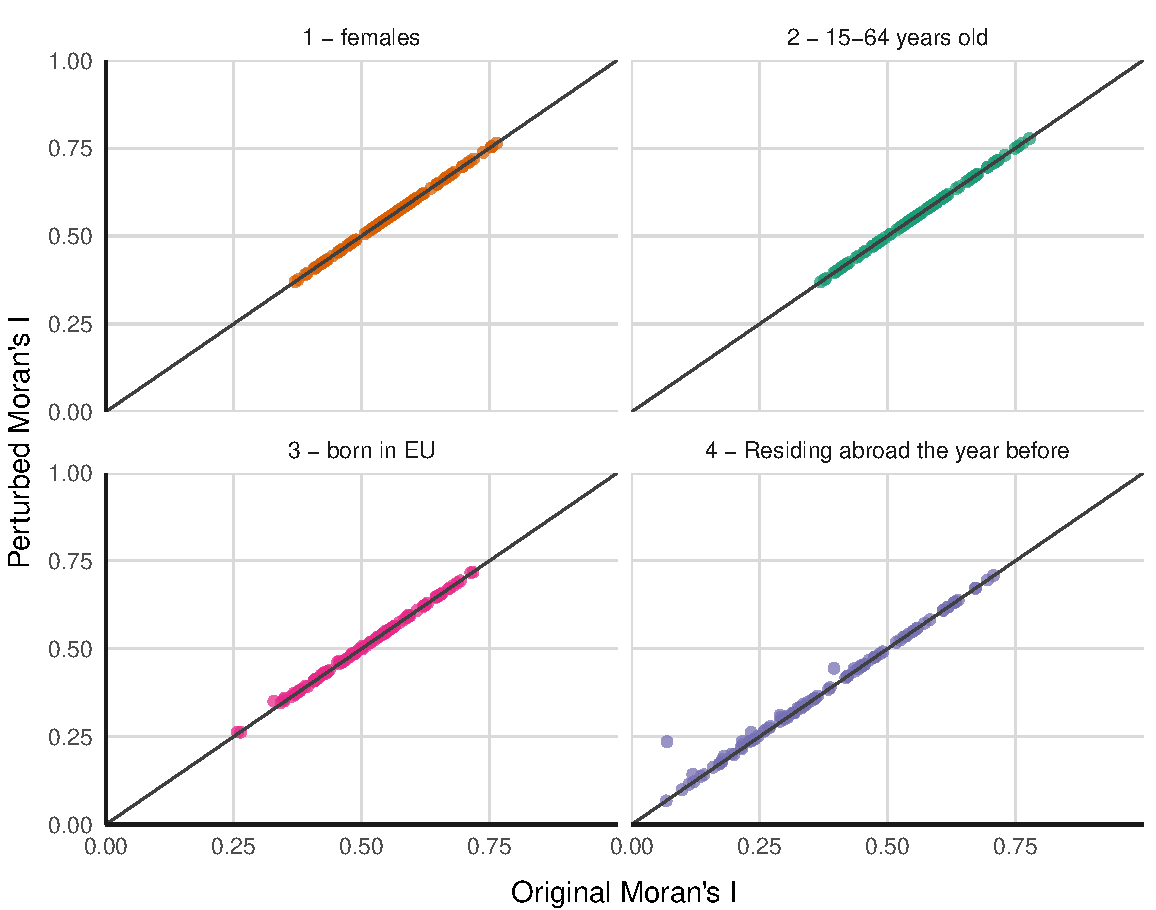
\includegraphics[width=\linewidth]{figures/Quadtree/carr_1km_moran_depts_4var_en_fix.pdf}
    \caption{Moran's $\mathcal{I}$ before and after treatment for several attributes, computed at the department level, departments being built from $1$~km tiles.}
    \label{fig:moran-depts}
\end{figure}

\newpage

